\chapter{Ausblick}
\label{ausblick}

Die vorgestellten und entwickelten Ansätze zum Lernen auf Graphen im zweidimensional euklidischen Raum wurden in dieser Arbeit über einer Klassizierung auf Graphrepräsentationen von Bildern evaluiert.
Sie lassen sich jedoch auch mühelos auf andere Probleme wie \zB{} der Objekterkennung oder der Segmentierung anwenden.
Dabei sind ebenso völlig andere als die in dieser Arbeit präsentierten Anwendungsgebiete denkbar, denn die einzige Einschränkung der Graphen für die Benutzung der entwickelten Faltungsoperatoren ist die eindeutige oder zumindest relative Positionierung seiner Knoten zueinander im Raum.
So lassen sich solche Graphen \bspw{} über Karten oder Straßennetze gewinnen, deren Eingabe in die vorgestellten Netzarchitekturen vielversprechende Möglichkeiten offenbaren.

Zum Abschluss dieser Arbeit wird ein Ausblick zu denkbaren Erweiterungen vorgestellt, für deren Erforschung an dieser Stelle der Platz fehlt.

\paragraph{Erweiterung auf den dreidimensionalen Raum}
\label{dredimensionale_erweiterung}

Alle Faltungsansätze in dieser Arbeit wurden lediglich auf Graphen im zweidimensionalen Raum betrachtet.
Dabei ist es aber ebenso vorstellbar, diese Ansätze auf den dreidimensionalen Raum auszuweiten.
In diesem Fall besitzt ein Graph $\gls{G} = \left(\gls{V}, \gls{E}, \gls{p}\right)$ eine Positionsfunktion $\gls{p} \colon \gls{V} \to \gls{R}^3$, die den Knoten jeweils drei Koordinaten zuordnet.
Die implizit gegebene Winkelfunktion seiner Kanten $\gls{winkel} \colon \gls{V} \times \gls{V} \to {\left[0, 2\pi\right]}^2$ bildet damit folglich auf zwei Winkel ab.
Insbesondere der spektrale Faltungsoperator, der in Kapitel~\ref{bspline} mit Hilfe einer polynomiellen Approximation über B-Spline-Kurven erweitert wurde, erlernt nun eine Repräsentation einer geschlossenen Fläche anstatt einer Kurve, die mittels der \emph{Tensorproduktkonstruktion} über zwei Basisfunktionen konstruiert werden kann~\cite{gm}.
Eine Implementierung \bzw{} Erweiterung dieser Ansätze auf den dreidimensionalen Raum erlaubt damit insbesondere das Lernen auf Polygonnetzen und folglich auch auf dreidimensionalen Objekten.

\paragraph{Entfernung irrelevanter Knoten}
\label{entfernung_irrelevanter_knoten}

In den Graphrepräsentationen von Bildern können bei der Benutzung der Quickshift-Segmentierung Knoten vereinzelnd einen extrem hohen Knotengrad aufweisen (\vgl{} \zB{} Tabelle~\ref{tab:mnist}).
Das ist insbesondere dann der Fall, wenn Knoten eine große einheitliche Fläche des Bildes abdecken (\zB{} einen einfarbigen Hintergrund) und folglich an dessen Segmenträndern viele benachbarte Pixel anliegen.
Eine Faltung auf diesen Knoten besitzt so gut wie keine lokale Aussage, sodass dessen Nutzen für ein neuronales Netzes fraglich oder gar hinderlich ist.
Es erscheint sinnvoll, diese Knoten in einem weiteren Vorverarbeitungsschritt über einer zuvor definierten Strategie zu entfernen.
Abbildung~\ref{fig:knotenentfernung} illustriert eine mögliche irrelevante Knotenentfernung anhand eines Bildes aus dem \gls{MNIST}-Datensatz.
\begin{figure}[t]
\centering
\subfigure[Ursprungsgraph]{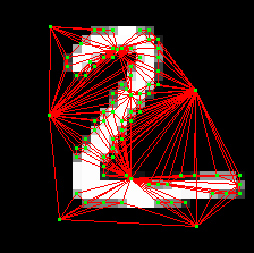
\includegraphics[scale=0.5]{bilder/knotenentferung_1}}
\hspace{1cm}
\subfigure[Knotenentfernung]{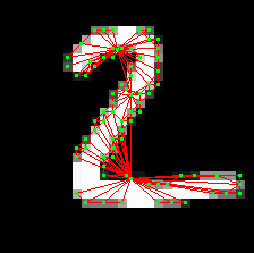
\includegraphics[scale=0.5]{bilder/knotenentferung_2}}
\caption[Entfernung irrelevanter Knoten]{Illustration der Entfernung irrelevanter Knoten eines Graphen, der über Quickshift eines Bildes aus dem \gls{MNIST} Datensatz gewonnen wurde.
(a) zeigt den Ursprungsgraphen der Segmentierung, wohingegen der Graph in (b) die irrelevanten Knoten, die den Hintergrund beschreiben, entfernt.}
\label{fig:knotenentfernung}
\end{figure}

Dabei lassen sich zwischen datensatzspezifischen und -unspezifischen Strategien unterscheiden.
Auf dem \gls{MNIST} Datensatz können \zB{} alle Knoten entfernt werden, die einen schwarzen Farbwert oder eine (relativ) große Fläche aufweisen.
Eine allgemeinere Vorgehensweise ist die Knotenentfernung basierend auf einem (relativen) Grenzwert seiner Knotengrade.
Bei der bloßen Entfernung von Knoten aus einem Graphen läuft man jedoch Gefahr, dass dieser nun möglicherweise isolierte Knoten \bzw{} mehrere Zusammenhangskomponenten besitzt.
Insbesondere die Poolingoperation sowie die Faltung basierend auf den \glspl{GCN} erfordern jedoch zusammenhängende Graphen.
Ein Test mit Hilfe des zweiten Eigenwerts der Laplace-Matrix zeigt, dass die Knotenentfernung basierend auf ihren Farbwerten für Graphen, die über Quickshift aus dem \gls{MNIST}-Datensatz generiert wurden, in $99.9\%$ der Fällen einen zusammenhängenden Graphen erhält, wohingegen für eine Knotenentfernung auf Basis ihrer Knotengrade dies nur noch für $45.4\%$ der Graphen der Fall ist.
Es lassen sich jedoch die beiden nächsten zueinander liegenden Knoten unterschiedlicher Zusammenhangskomponenten über eine Kante verbinden, bis der Graph wieder zusammenhängend ist.

\paragraph{Spatial Pyramid Pooling}
\label{spatial_pyramid_pooling}

Eine Alternative zu der verwendeten Durchschnittsbildung zwischen Faltungs- und vollverbundener Schicht, die für die Implementierung der spektralen Netzarchitektur auf Graphen mit dynamischer Knotengröße benutzt wurde (\vgl{} Kapitel~\ref{spektrale_netzarchitektur}), ist das \emph{\gls{SPP}}~\cite{spp}.
Die \gls{SPP}-Schicht erhält entgegen der Durchschnittsbildung räumliche Informationen, indem über einer Menge räumlicher Gruppierungen unterschiedlicher Auflösungen \emph{gepoolt} wird, sodass sich als Endresultat ein Vektor fester Größe ergibt (\vgl{}~\cite{spp}).
Ein modifizierter Ansatz dieses Algorithmus auf Graphen erfordert demnach die Vergröberung der Graphen auf deren gemeinsame kleinste Größe (Vielfaches von zwei) mit möglicherweise unterschiedlich vielen Ebenen.
Damit ist die Verwendung einer \gls{SPP}-Schicht mit weitaus mehr Berechnungsaufwand verbunden, dessen Qualität aufgrund der Translationsinvarianz von Adjazenzmatrizen erst zu evaluieren ist.

Eine weitere Alternative ist die Verwendung eines \emph{Attentation}-Mechanismus, der beispielsweise in \emph{\glspl{RNN}} zum Einsatz kommt~\cite{attentation}.

\paragraph{Effiziente GPU-Implementierung}
\label{gpu_implementierung}

Die Laufzeiten der vorgestellten Faltungsoperatoren können derzeit, obgleich einer kleineren Eingabegröße, nicht mit den Laufzeiten der klassichen Faltung auf Bildern konkurrieren.
Der klassische Faltungsoperator besitzt eine für die GPU höchst optimierte batchweise Implementierung, wohingegen die Graphimplementierung aufgrund der Limitierung dünnbesetzter Tensoren auf genau zwei Dimensionen dies nicht leisten kann.
Für die Verarbeitung eines \mbox{Batches} muss folglich über jeden Graphen einzeln iteriert werden, sodass die Vorteile der Nutzung einer GPU \bzgl{} ihrer Parallelisierungsmechanismen verloren gehen.
Eine Möglichkeit, diese Schwäche zu umgehen, ist die batchweise Darstellung der Adjazenzmatrizen $\mathcal{A} \coloneqq {\left\{\gls{A}_m\right\}}_{m=1}^M$ über genau eine dünnbesetzte Matrix, sodass die Adjazenzmatrizen diagonalbasiert angeordnet sind, \dhe{}
\begin{equation*}
  \mathcal{A} \coloneqq \begin{bmatrix}
  \gls{A}_1 & & \ma{0}\\
  & \ddots & \\
  \ma{0} & & \gls{A}_M
  \end{bmatrix},
\end{equation*}
und folglich einheitlich verarbeitet werden können.
Die Optimierung dieses Ansatzes bleibt ein interessantes Forschungsgebiet für weiterführende Arbeiten.
